\documentclass{article}
\usepackage[utf8]{inputenc}
\usepackage[T1]{fontenc} 
%\usepackage[french]{babel}
\usepackage{charter} 
\usepackage{graphicx} 
\usepackage{amsmath}
\usepackage{amsthm}
\usepackage{amsfonts}
\usepackage{geometry}
\usepackage{cancel}
\usepackage{enumerate}
\usepackage{stmaryrd}
\usepackage{mathrsfs}
\usepackage{amssymb}
\geometry{hmargin=2.7cm,vmargin=2.5cm}

\usepackage{lastpage}
\usepackage{fancyhdr}
\pagestyle{fancy}
\renewcommand{\headrulewidth}{0pt}
\renewcommand{\footrulewidth}{0.5pt}
\fancyhead[L]{}
\fancyhead[R]{}
\fancyfoot{}
\fancyfoot[L]{RS -- Quentin CHAN-WAI-NAM}
\fancyfoot[R]{\thepage/\pageref{LastPage}}

\fancypagestyle{plain}{
	\renewcommand{\headrulewidth}{0pt}
	\renewcommand{\footrulewidth}{0.5pt}
	\fancyhead[L]{}
	\fancyhead[R]{}
	\fancyfoot{}
	\fancyfoot[L]{RS -- Quentin CHAN-WAI-NAM}
	\fancyfoot[R]{\thepage/\pageref{LastPage}}
}

\usepackage{animate}

\def\thesubsection{\thesection.\alph{subsection}}

\makeatletter
\def\thm@space@setup{%
  \thm@preskip=15pt \thm@postskip=15pt
}
\makeatother

\linespread{1.3}

\newcommand{\abs} [1] {\left| #1 \right|}
\newcommand{\scal}[2]{\left\langle #1 , #2 \right\rangle}
\newcommand{\dif}[0]{\text{\:d}}
\newcommand{\Dpar}[2]{\frac{\partial#1}{\partial#2}}

\newcommand{\ceil}[1]{\lceil#1\rceil}
\newcommand{\floor}[1]{\lfloor#1\rfloor}

\newcommand{\Four}[1]{\widehat{#1}}

\newcommand{\norm}[1]{\left\lVert#1\right\rVert}

\def\R{\mathbb{R}}
\def\Z{\mathbb{Z}}
\def\N{\mathbb{N}}
\def\e{\text{e}}
\def\d{\text{d}}
\def\Re{\text{Re}}

\def\Per{\text{Per}\,}
\def\Ker{\text{Ker}\,}
\def\Im{\text{Im}\,}

\def\Ind{\mathbf{1}}

% Width of the EPIs
\def\epiWidth{0.8}

\newcommand{\Binom}[2]{\begin{pmatrix} #1 \\ #2 \end{pmatrix}}

\newcommand{\vect}[1]{\mathbf{#1}}

%%%%%%%%%%%%%%%%%%%%%%%%%%%%%%%%%%%%%%%%%%%%%%%%%%%%%%%%%%%%%%%%%%%%%%%%%%%%%%%%%%%%%%%%%%%%%%%%

\title{RS: Epipolar Plane Image Analysis\\Application to SkySat videos}
\date{\today}
\author{Quentin CHAN-WAI-NAM}

\theoremstyle{definition}
\newtheorem{question}{}

\begin{document}
\maketitle


\section{Choice of the article and objective}


We first investigated two different articles that describe two different methods for estimating depths maps from videos.
\begin{itemize}
 \item \cite{art:perez13:tvl1} describes an algorithm that estimates the optical flow given two images using a global optimization scheme minimizing a data attachment term and a regularization using the total variation of the flow. The idea is that the brightness $I$ of single points along their trajectories should be constant in time, leading to the optical flow constraint equation
 \[ \nabla I \cdot \vect{u} + \Dpar{I}{t} = 0 \]
 where $\vect{u}$ is the optical flow (the velocity vector field). The article then introduces a regularization on $\vect{u}$ (its total variation) and reformulates the problem in order to adapt to discrete sequences of images so that the attachent term consists in minimizing some $L^1$ term. In order to solve the subsequent global optimization problem, the authors propose a numerical scheme based on alternate optimization scheme. Finally, the authors investigate the influence of the several parameters of the algorithm -- noticeably the weight $\lambda$ of the data attachment term -- on the precision of the estimation of the optical flow and the sensitivity to noise.
 
 In our case, the optical flow computed with this algorithm could be interpreted as some disparity measurement. An interesting point is that the computation of the optical flow can be done on any pair of images, even if not rectified.
 
 \item \cite{art:kim13:lfields} describes a method for computing precise and exhaustive depth maps using ``light fields'', that is a dense set of images captures along a linear path. By concatenating one line of the rectified images together, one obtains an ``epipolar-plane image'' (EPI), in which a single scene point appears as a linear trace which slope is related to its distance to the camera. Thus, by estimating these slopes, one can reconstruct the depth of each point of the scene.
 
 The authors use very high definition images, so that the article includes several implementation details in order to ensure computational feasibility, both in terms of space (sparse representation of light fields) and computational power. For instance, they prefer local optimization near object boundaries and propagation to nearby areas in a fine-to-coarse approach to global optimization on the whole image. In the end, the method seems relatively fast, precise and robust to inconsistencies and outliers like noise or temporary occlusions.
\end{itemize}


We chose to work on the latter article. The objective of the project is then to implement the method presented by Kim et al. in \cite{art:kim13:lfields} and investigate how it performs with videos taken from SkySat. We will first investigate the case in which the images from the video are pre-rectified. Then we will investigate more complicated situations, for instance increasing the density of the images and considering non-pre-rectified sequences.


\section{Sample EPIs from Skysat (step 18)}


\paragraph{Test} \verb#test_build_row_epi_skysat_rectified_18.cpp#.


We first write codes to compute and display EPIs. We investigate possible artefacts that appear in the EPIs extracted from the rectified images of Skysat, with step $18$.


\begin{figure}[ht]
  \centering
  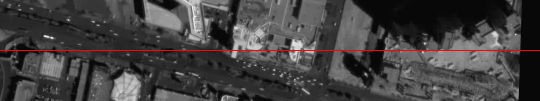
\includegraphics[width=\epiWidth\textwidth]{images/1519991014186_1st.png}\\
  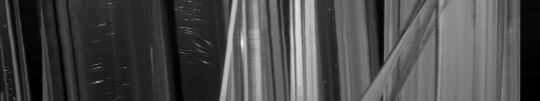
\includegraphics[width=\epiWidth\textwidth]{images/1519991014186_epi.png}
  \caption{Row 600 -- We can see that the cars produce some artefacts.}
\end{figure}


\begin{figure}[ht]
  \centering
  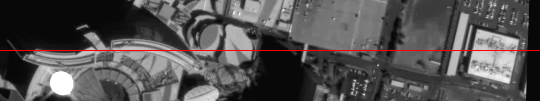
\includegraphics[width=\epiWidth\textwidth]{images/1519991030012_1st.png}\\
  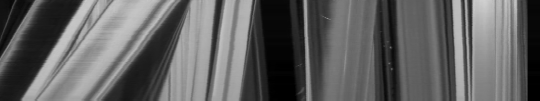
\includegraphics[width=\epiWidth\textwidth]{images/1519991030012_epi.png}
  \caption{Row 380 -- The high building has a very steep slope. The color of some points seem to vary in time (due to changes in illumination and shading). We also note some strong occlusions.}
\end{figure}


\begin{figure}[ht]
  \centering
  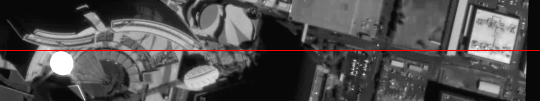
\includegraphics[width=\epiWidth\textwidth]{images/1519991772641_1st.png}\\
  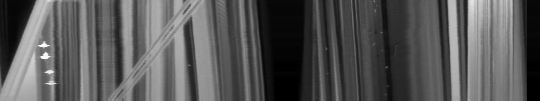
\includegraphics[width=\epiWidth\textwidth]{images/1519991772641_epi.png}
  \caption{Row 400 -- The specular reflexions produce artefacts.}
\end{figure}


\begin{figure}[ht]
  \centering
  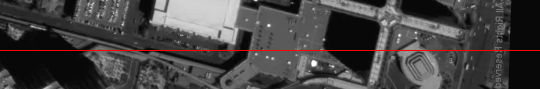
\includegraphics[width=\epiWidth\textwidth]{images/1519992108606_1st.png}\\
  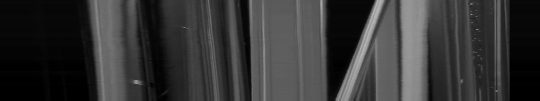
\includegraphics[width=\epiWidth\textwidth]{images/1519992108606_epi.png}
  \caption{Row 920 -- The shadows produce empty black zones.}
\end{figure}


\clearpage
\section{First rough estimation of the disparities}


\paragraph{Principle} We apply a very simplified version of the first step of the ``fine to coarse'' approach of \cite{art:kim13:lfields}: we take some EPI $E$ corresponding to a fixed $v$, which dimensions are $S$ along the rows and $U$ along the columns. We work only on one line of this EPI (the center line, at $\widehat{s} = S / 2$. Let $d_\text{list} = \left\{d_1, \cdots, d_D \right\}$ be a search set of disparities. We compute the set of radiances $\mathcal{R}$ for all couples $(u, d)$:
\[ \mathcal{R}(u, d) = \left\{ E(u + (\widehat{s} - s) d, s) \; | \; s = 0 \cdots S-1 \right\}. \]

We then compute a score $S(u, d)$ defined as:
\[ S(u, d) = \frac{1}{\abs{\mathcal{R}(u, d)}} \sum_{\mathbf{r} \in \mathcal{R}(u, d)} K(\mathbf{r} - \overline{\mathbf{r}})\]
where $\mathbf{r}$ can be a float, or in the case of the images of the mansion, a tricolor vector, and $K$ is a ``kernel''. We choose the kernel presented in the article, i.e.
\[ K(\mathbf{r}) = \left\{ 
\begin{array}{l}
1 - \norm{\mathbf{r} / h}^2 \qquad \text{if $\norm{\mathbf{r} / h} < 1$} \\
0 \qquad \text{else}                            
\end{array} \right. .
\]
We name this kernel the ``bandwidth kernel'' (and we take $h = 0.2$ arbitrarily for now).

$\overline{\mathbf{r}}$ is a parameter that depends on $(u, d)$: following the article, we perform a truncated mean-shift algorithm (10 iterations), with $\overline{\mathbf{r}}_0 = E(u, \widehat{s})$ and
\[ \overline{\mathbf{r}} \leftarrow \frac{\sum_{\mathbf{r} \in \mathcal{R}(u, d)} K(\mathbf{r} - \overline{\mathbf{r}}) \mathbf{r}}{\sum_{\mathbf{r} \in \mathcal{R}(u, d)} K(\mathbf{r} - \overline{\mathbf{r}})}\]
prior to the computation of $S(u, d)$.

Finally, for each $u$, we select the $d$ with the best score. We discard scores $< 0.01$ ; if no score is available, then we take $d=0$. We apply a linear median filter (along the $u$ dimension only for now) on the resulting values $d$ (we choose a filter size of $5$).

We propagate the disparities from $\widehat{s}$ to the other $s$ simply by drawing the depths along the lines $u + (\widehat{s} - s)d$ and respecting the occlusions (a point with higher disparity will be ``occluding'' a point with a lesser disparity).


\paragraph{Technical difficulties} A line defined by $(u + (\widehat{s} - s) d, s)$ will very certainly end up going out of the image. Moreover, these coordinates are not integer coordinates. We thus take the following decisions:
\begin{itemize}
 \item Values outside of the image are considered \emph{nan} and not taken into account in $\mathcal{R}(u, d)$.
 \item We have yet to decide on some proper interpolation method for computing non-integer values of $E$. For now, we choose a simple linear interpolation along the line $E(u, \cdot)$.
 \item The complexity of the algorithm increases quite a bit with the dimensions of the image. We might implement the algorithms using GPUs, but now we use tricks like OpenMP.
\end{itemize}
We also created a template code so as to be able to adapt to different data types for $E$ (e.g. \verb#float#, \verb#uint#, \verb#cv::Vec3b#...).


\paragraph{Results} We choose $d_\text{list} = \left\{-2.0, -2.05, \cdots, 3.95, 4.0\right\}$. We end up with the following results. We expect to improve these using confidence scores $C_e$ as in the article for instance, and computing depths for more $s$ than only $\widehat{s}$.


\begin{figure}[ht]
  \centering
  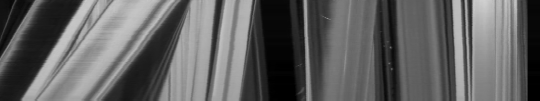
\includegraphics[width=\epiWidth\textwidth]{images/1520204861279_epi.png}\\
  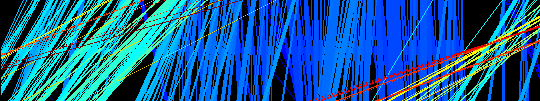
\includegraphics[width=\epiWidth\textwidth]{images/1520204861279_epi_colored.png}
  \caption{Skysat rectified, row 380. We note some parasite extreme lines. We interpret these as parasite low-confidence slopes.}
\end{figure}


\begin{figure}[ht]
  \centering
  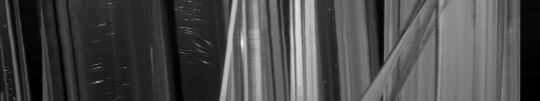
\includegraphics[width=\epiWidth\textwidth]{images/1520205010590_epi.png}\\
  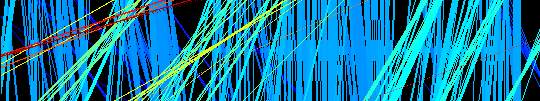
\includegraphics[width=\epiWidth\textwidth]{images/1520205010590_epi_colored.png}
  \caption{Skysat rectified, row 600. Cars do not seem to make a huge difference, but homogeneous zones are not well handled.}
\end{figure}


\begin{figure}[ht]
  \centering
  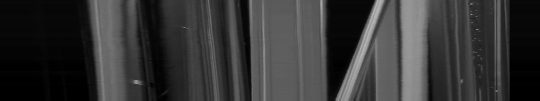
\includegraphics[width=\epiWidth\textwidth]{images/1520205074004_epi.png}\\
  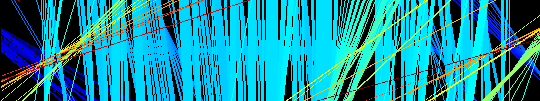
\includegraphics[width=\epiWidth\textwidth]{images/1520205074004_epi_colored.png}
  \caption{Skysat rectified, row 920. As expected, the algorithm does not work well in the shadows.}
\end{figure}


\begin{figure}[ht]
  \centering
  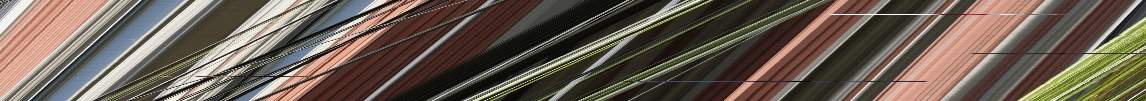
\includegraphics[width=\epiWidth\textwidth]{images/1520202945623_epi.png}\\
  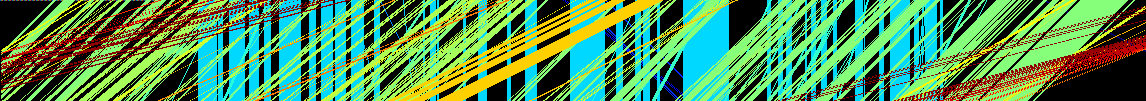
\includegraphics[width=\epiWidth\textwidth]{images/1520202945623_epi_colored.png}
  \caption{Mansion sample (undersized to $1146\times 720$), row 380.}
\end{figure}


\clearpage
\section{After scaling, confidence threshold}


In fact, it is better to scale the images between $0.0$ and $1.0$ before processing. We do the following:
\begin{itemize}
 \item If the provided image is of type \verb#uchar#, i.e. values are in $0 \cdots 255$, then we scale by $255$.
 \item Else, we scale by the max over all the channels.
\end{itemize}
Results are much cleaner (Figures \ref{fig:wscaling:skysat:380}, \ref{fig:wscaling:mansion:380}).


\begin{figure}[ht]
  \centering
  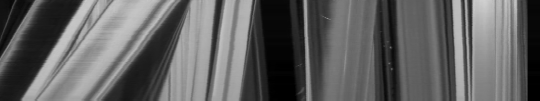
\includegraphics[width=\epiWidth\textwidth]{images/1520334265034_epi.png}\\
  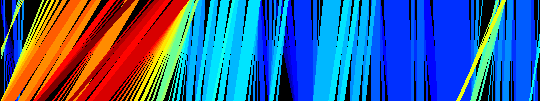
\includegraphics[width=\epiWidth\textwidth]{images/1520334265034_epi_colored.png}
  \caption{Skysat rectified, with scaling, row 380.}
  \label{fig:wscaling:skysat:380}
\end{figure}


\begin{figure}[ht]
  \centering
  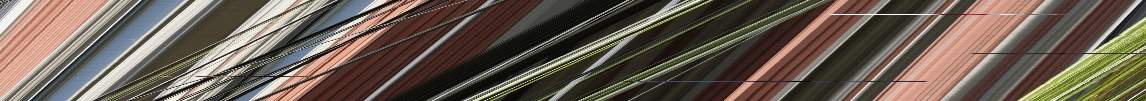
\includegraphics[width=\epiWidth\textwidth]{images/1520334290628_epi.png}\\
  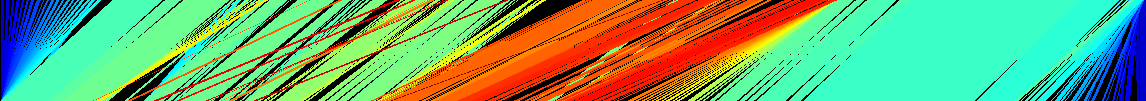
\includegraphics[width=\epiWidth\textwidth]{images/1520334290628_epi_colored.png}
  \caption{Mansion sample, with scaling, (undersized to $1146\times 720$), row 380.}
  \label{fig:wscaling:mansion:380}
\end{figure}


If we add the confidence measures: confidence edge $C_e$ and final confidence $C_d$ such that:
\begin{align}
 C_e (u, \widehat{s}) &= \sum_{u' \in \mathcal{N}(u, \widehat{s})} \norm{E(u, \widehat{s}) - E(u', \widehat{s})}^2 \\
 C_d (u, \widehat{s}) &= C_e (u, \widehat{s}) \norm{\max_d S(u, d) - \mathrm{mean}_d S(u, d)}
\end{align}
we obtain the results presented in Figures \ref{fig:wconf:skysat:380}, \ref{fig:wconf:mansion:380}. We disable the median filter along d's for these tests.


\begin{figure}[ht]
  \centering
  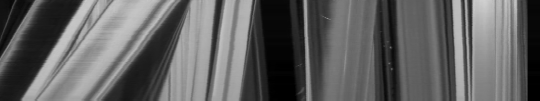
\includegraphics[width=\epiWidth\textwidth]{images/1520354672022_epi.png}\\
  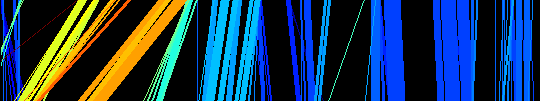
\includegraphics[width=\epiWidth\textwidth]{images/1520354672022_epi_colored.png}
  \caption{Skysat rectified, with scaling and score threshold, no median filter, row 380.}
  \label{fig:wconf:skysat:380}
\end{figure}


\begin{figure}[ht]
  \centering
  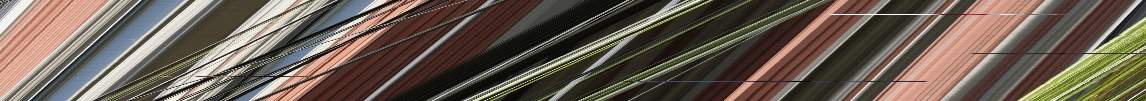
\includegraphics[width=\epiWidth\textwidth]{images/1520354635991_epi.png}\\
  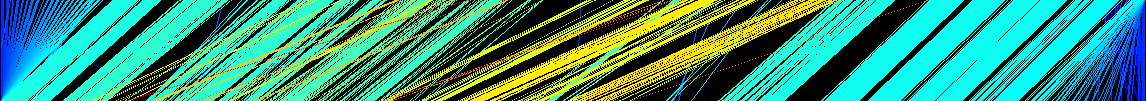
\includegraphics[width=\epiWidth\textwidth]{images/1520354635991_epi_colored.png}
  \caption{Mansion sample, with scaling and score threshold, no median filter, (undersized to $1146\times 720$), row 380.}
  \label{fig:wconf:mansion:380}
\end{figure}


\begin{figure}[ht]
  \centering
  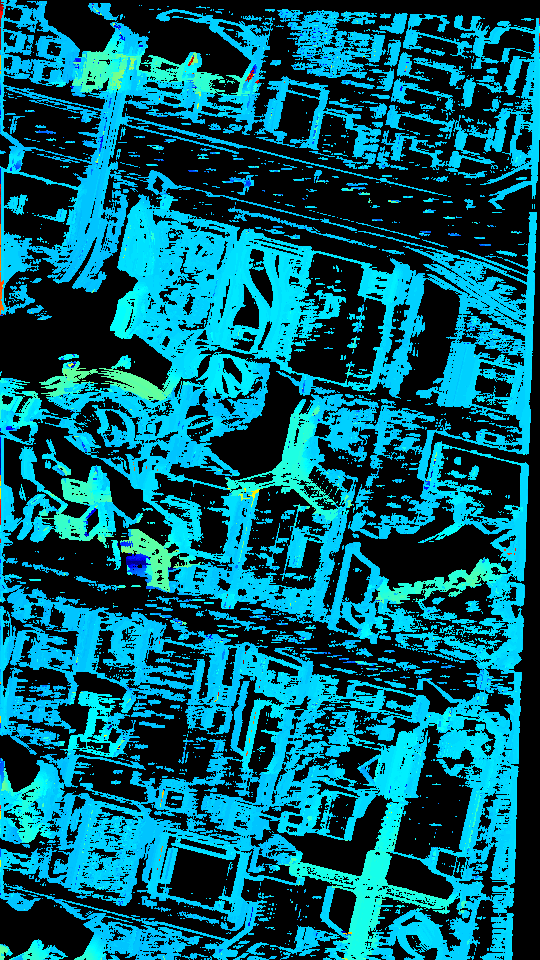
\includegraphics[width=0.35\textwidth]{images/1520423162502_dmap.png}
  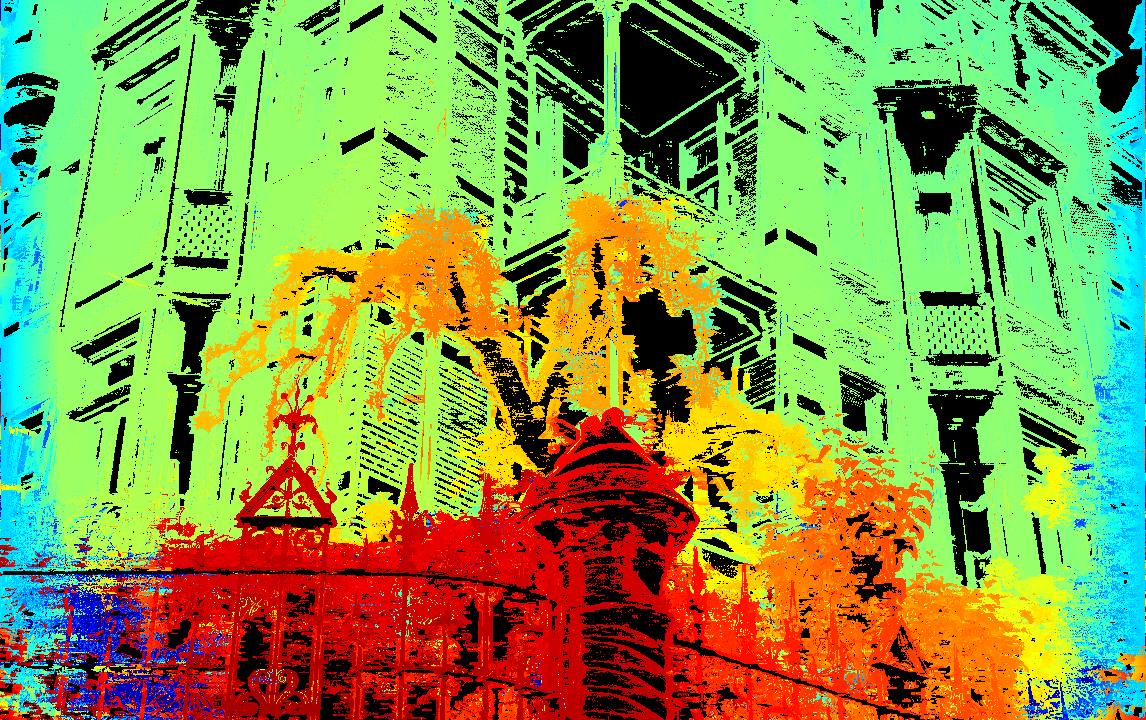
\includegraphics[width=0.7\textwidth]{images/1520438877175_dmap.png}
  \caption{Sample outputs depth maps where $C_e > 0.02$ (mansion [626 seconds] and Skysat [51 seconds] with 120 tested $d$ values between $-2.0$ and $4.0$, no median filter)}
  \label{fig:wconf:piles}
\end{figure}


\clearpage
\section{Selective median filter}

We implement and apply a median filter on the resulting disparity map $D$ along dimensions $u, v$ such that in the end, for a point $(u, v)$ such that $C_e (u, v) > 0.02$, the selected value $d_{u, v}$ is the median value of the set:
\[ \left\{ d_{u', v'} \; | \; (u', v') \in \mathcal{N}_{u, v}, \; C_e(u', v') > 0.02, \; \norm{E_{v}(\widehat{s}, u) - E_{v'}(\widehat{s}, u')} < 0.1 \right\}.\]

$\mathcal{N}_{u, v}$ is a neighbourhood of $(u, v)$ -- we select a square neighbourhood centered on $(u, v)$, of overall size $k$. The results are presented in Figures x, x.


\begin{figure}[ht]
  \centering
  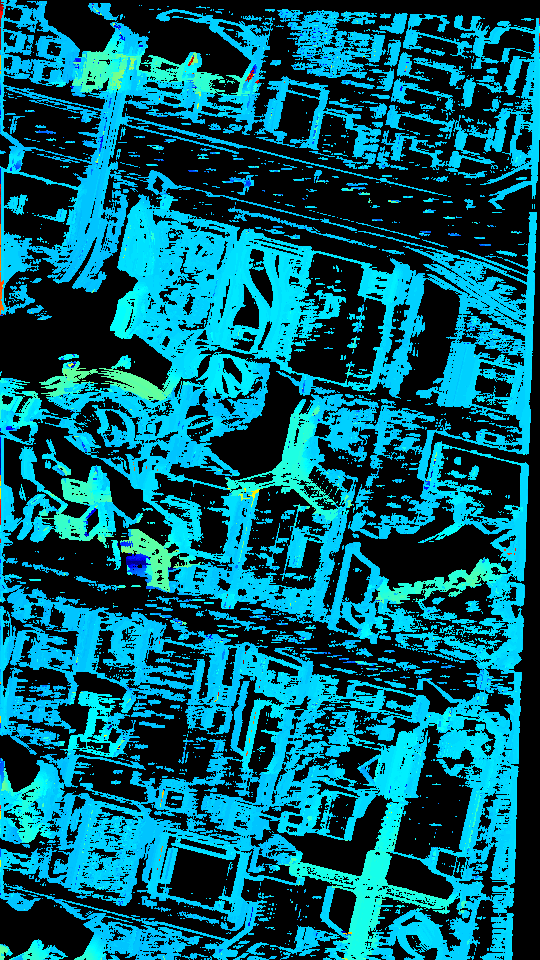
\includegraphics[width=0.3\textwidth]{images/1520620453023_dmap.png}
  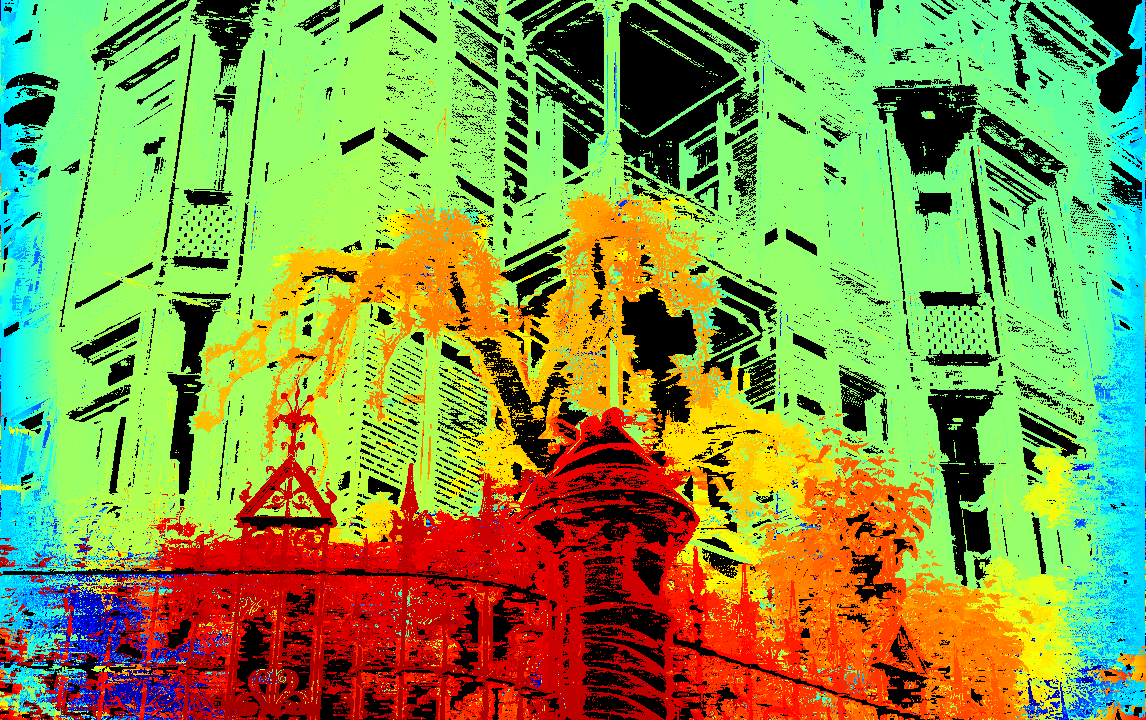
\includegraphics[width=0.6\textwidth]{images/1520620380080_dmap.png} \\
  
  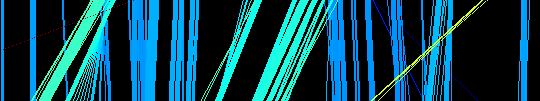
\includegraphics[width=0.3\textwidth]{images/1520620453023_epi_colored.png}
  
\includegraphics[width=0.6\textwidth]{images/1520618708656_epi_colored.png}
  \caption{Disparity map and sample epi after median filter, $k=1$ (no median)}
  \label{fig:median:1}
\end{figure}


\begin{figure}[ht]
  \centering
  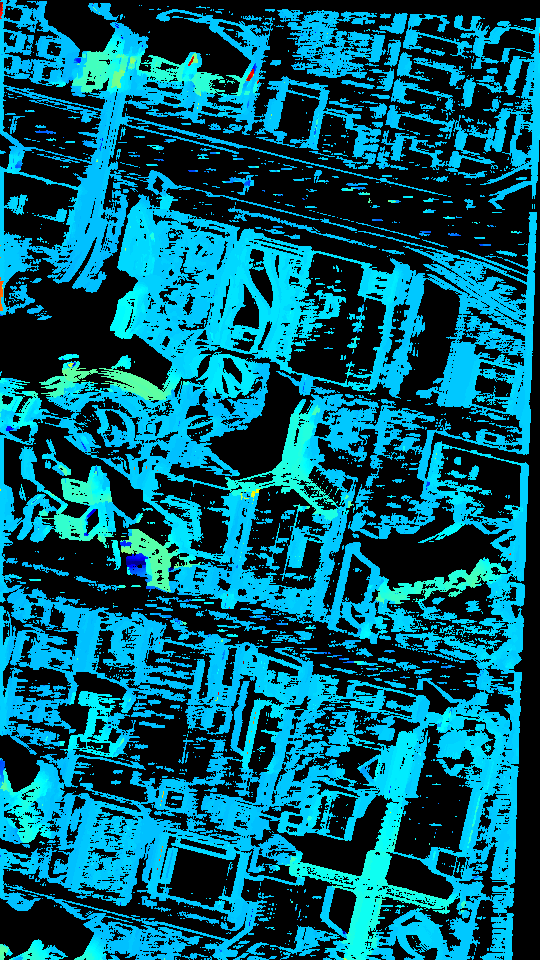
\includegraphics[width=0.3\textwidth]{images/1520617477650_dmap.png}
  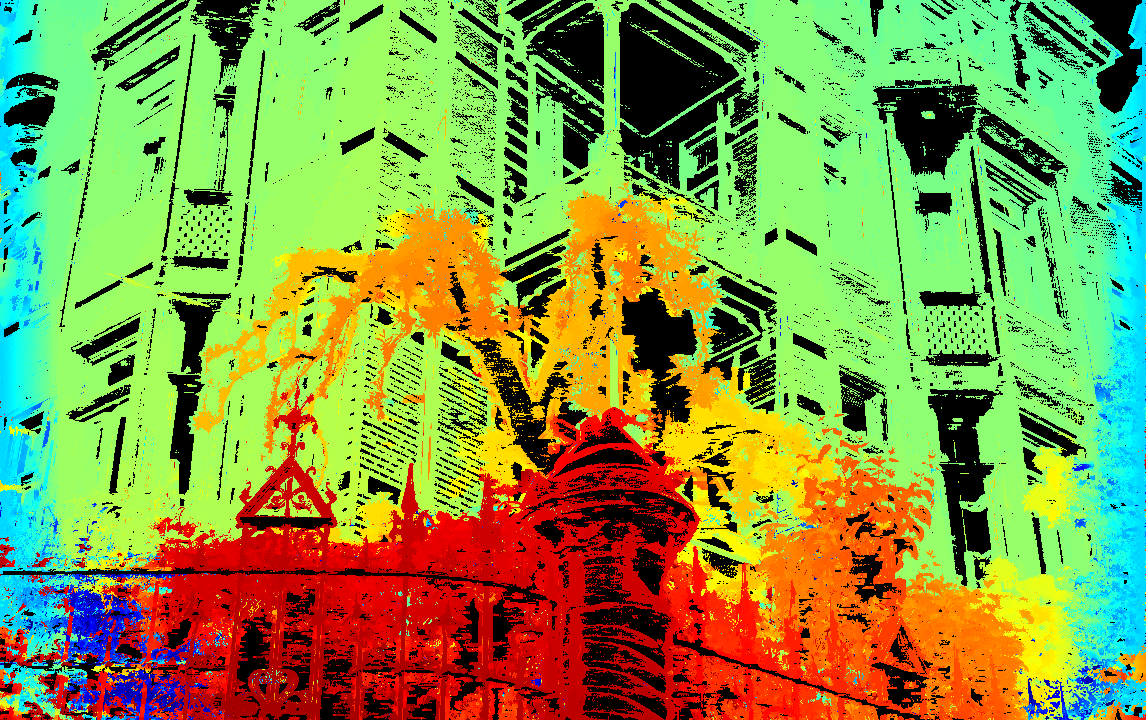
\includegraphics[width=0.6\textwidth]{images/1520618100513_dmap.png} \\
  
  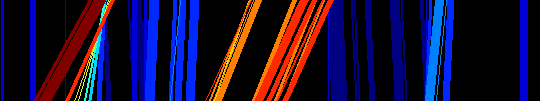
\includegraphics[width=0.3\textwidth]{images/1520617477650_epi_colored.png}
  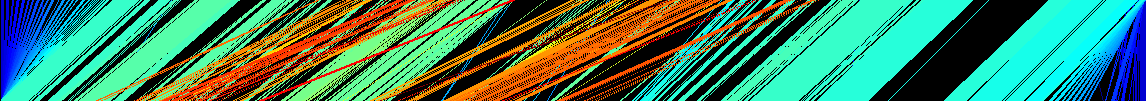
\includegraphics[width=0.6\textwidth]{images/1520618100513_epi_colored.png}
  \caption{Disparity map and sample epi after median filter, $k=5$}
  \label{fig:median:5}
\end{figure}


\begin{figure}[ht]
  \centering
  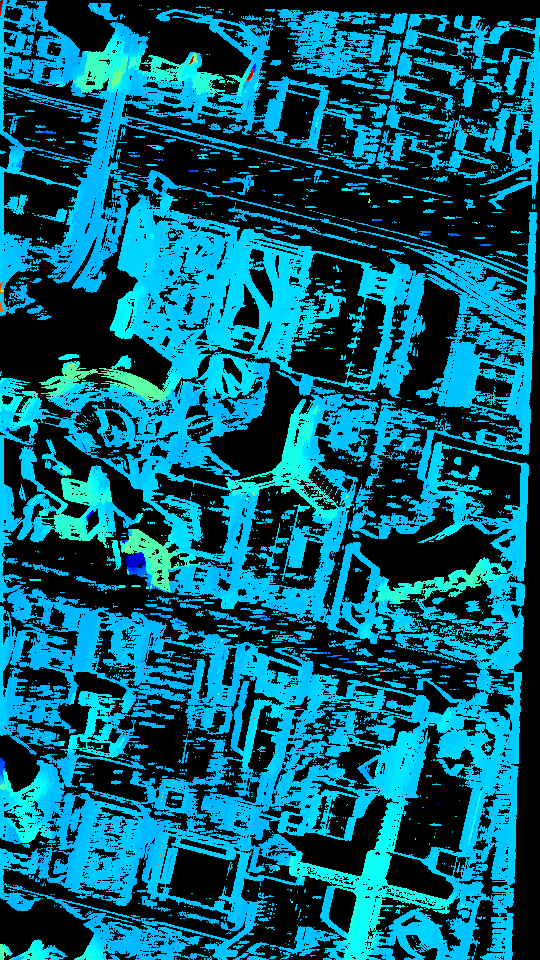
\includegraphics[width=0.3\textwidth]{images/1520617394231_dmap.png}
  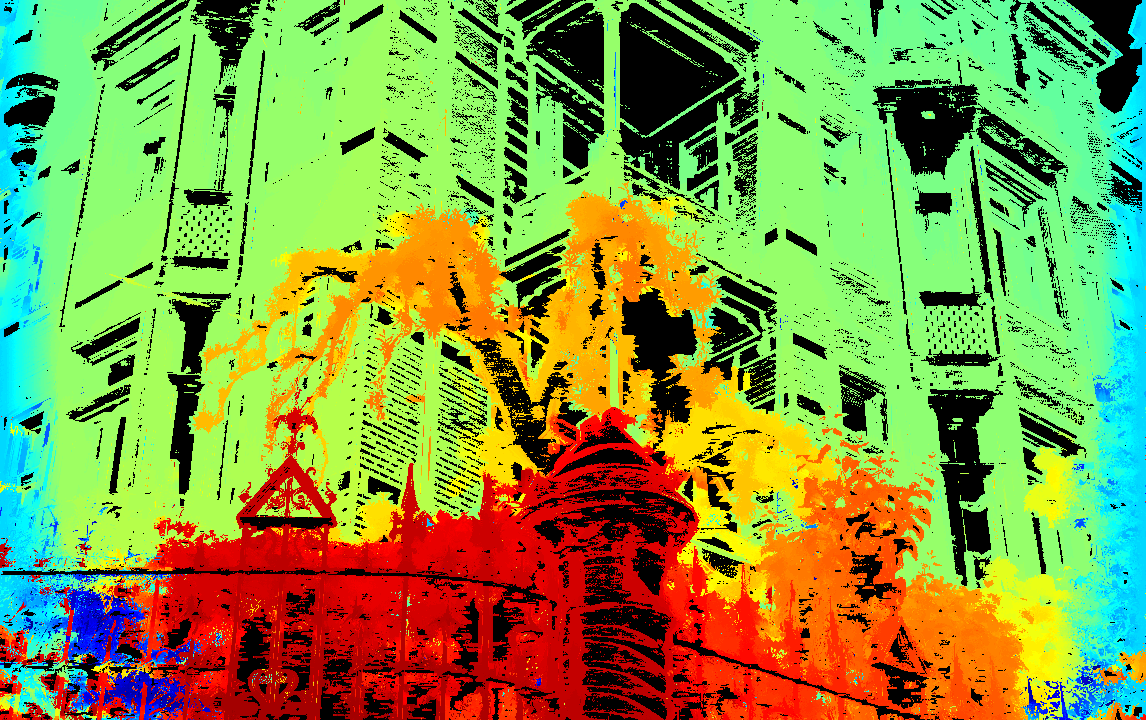
\includegraphics[width=0.6\textwidth]{images/1520618708656_dmap.png} \\
  
  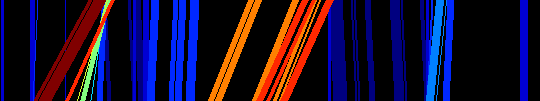
\includegraphics[width=0.3\textwidth]{images/1520617394231_epi_colored.png}
  
\includegraphics[width=0.6\textwidth]{images/1520618708656_epi_colored.png}
  \caption{Disparity map and sample epi after median filter, $k=11$}
  \label{fig:median:11}
\end{figure}


\clearpage
\section{Disparity propagation}


After computing the depths for the points $u$ with some fixed $(v, \widehat{s} = \max s / 2)$, and applying a median filter of size 5 along the $(u, v)$ axis, we apply the disparity propagation along the $s$ axis, using the following rules: we propagate the optimal disparity $d(u, \widehat{s})$ computed at $(u, \widehat{s})$ to a point $(u', s')$ (where $u' = u + (\widehat{s} - s') \times d(u, \widehat{s})$) if:
\begin{enumerate}
 \item $C_e(u, s) > 0.02$
 \item $C_e(u', s') > 0.02$
 \item $\norm{E(u', s') - E(u, \widehat{s})} < 0.1$
\end{enumerate}


In the article, the first rule would have rather been $C_d(u, s) > 0.1$. Yet, we found that in our examples, $C_d$ is very low for most of the points, resulting in almost no disparity being propagating, even with a low threshold on $C_d$. Thus, we accept to propagate depths at points at which the confidence in the value $d$ is low. This is to be investigated further.


After propagating the depths, following the article, we compute the remaining unknown depths at points $(u, s)$ where $C_e(u, s) > 0.02$ for increasing $\abs{\widehat{s} - s}$, and propagate at each step. This leads to decreased computation times:
\begin{itemize}
 \item For the Skysat sequence, instead of ~4500 seconds (if no propagation is done), the process takes 294 seconds.
 \item For the downsampled mansion sequence, instead of ~51000 seconds, the process takes 7371 seconds.
\end{itemize}


Some sample frames are presented in Figure \ref{fig:propagation}. Note that we corrected a bug that perturbated the disparity computation around the borders in the mansion sequence.


We also performed a propagation using the criterion $C_d(u, s) > 0.1$. This criterion depends on the magnitude of the scores $S$ ; and thus, it is dependant on the values of the EPI. We normalized the image (the different channels take values in $[0, 1]$, yet the criterion is still dependant on the number of channels ; the equivalent threshold on the Skysat sequence would be different). This led to the Figure \ref{fig:propagation:disp} after a computation time of 34164 seconds. It seems that there is more noise than on the previous experiment, but also that the points that are correct have a more precise $d$ estimation.


It also seems that contrary to the mansion image, there seem to be some more blur or less contrast on the images of the Skysat sequence, that result in less points having a high $C_d$ (i.e. the values $d$ computed are likely to be imprecise on this particular sequence).





\begin{figure}[ht]
  \centering
  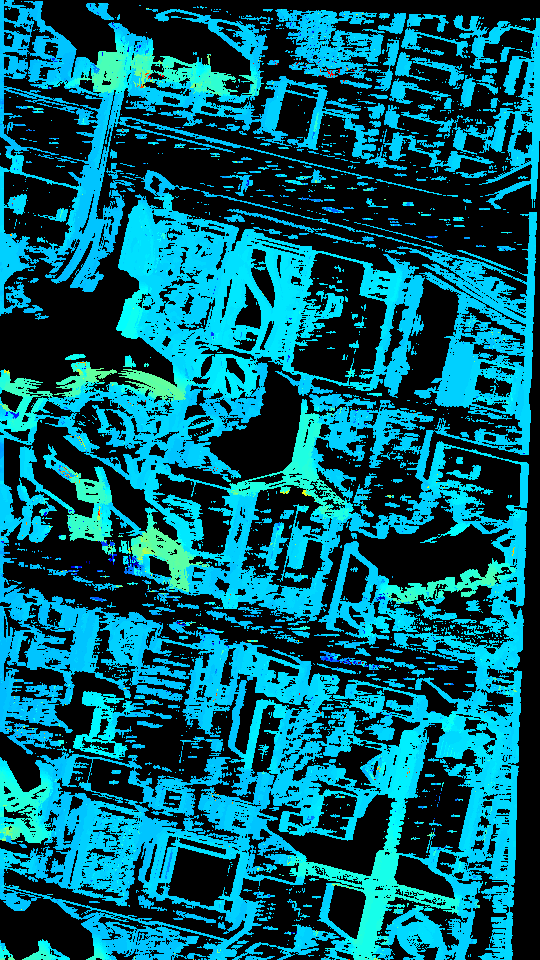
\includegraphics[width=0.3\textwidth]{images/1520867757275_dmap_025.png}
  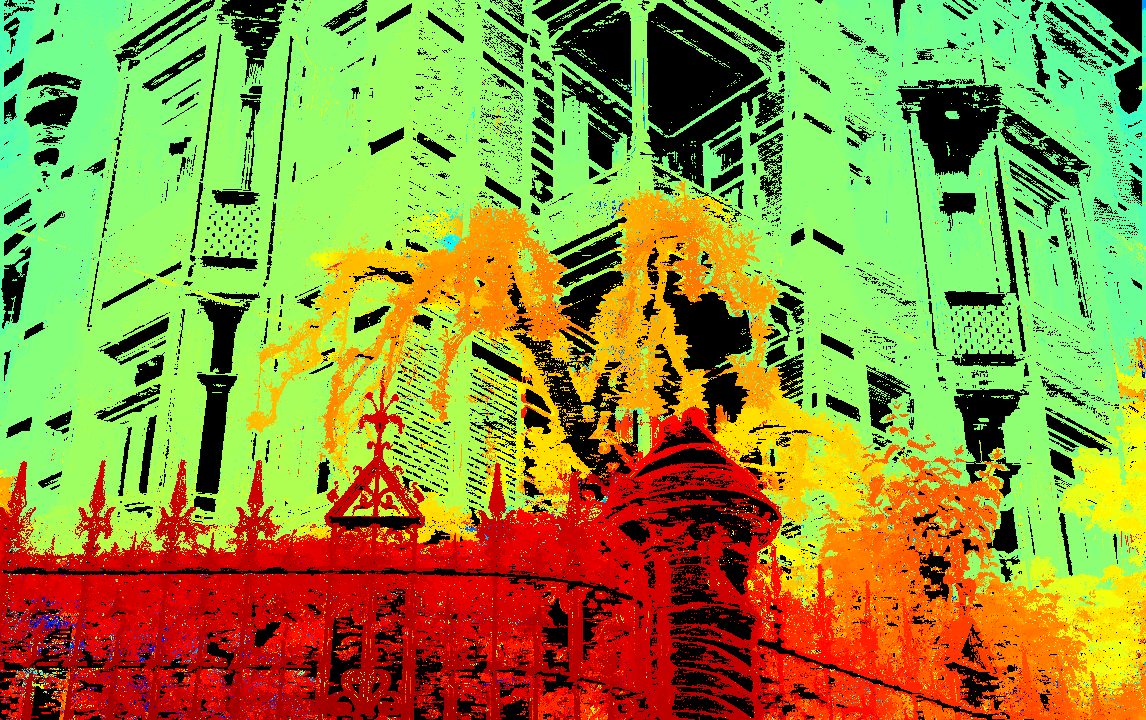
\includegraphics[width=0.6\textwidth]{images/1520877118843_dmap_025.png} \\
  
  
\includegraphics[width=0.3\textwidth]{images/1520867757275_epi_colored.png}
  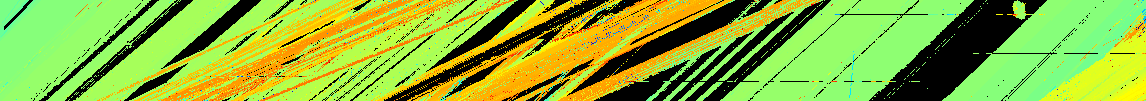
\includegraphics[width=0.6\textwidth]{images/1520877118843_epi_colored.png}
  \caption{Disparity map and sample epi after median filter, $k=5$, and propagation. The disparity maps correspond to frame 25, while the propagation originated from frame 50. The sample epis correspond to the midline of the image.}
  \label{fig:propagation}
\end{figure}


\begin{figure}[ht]
  \centering
  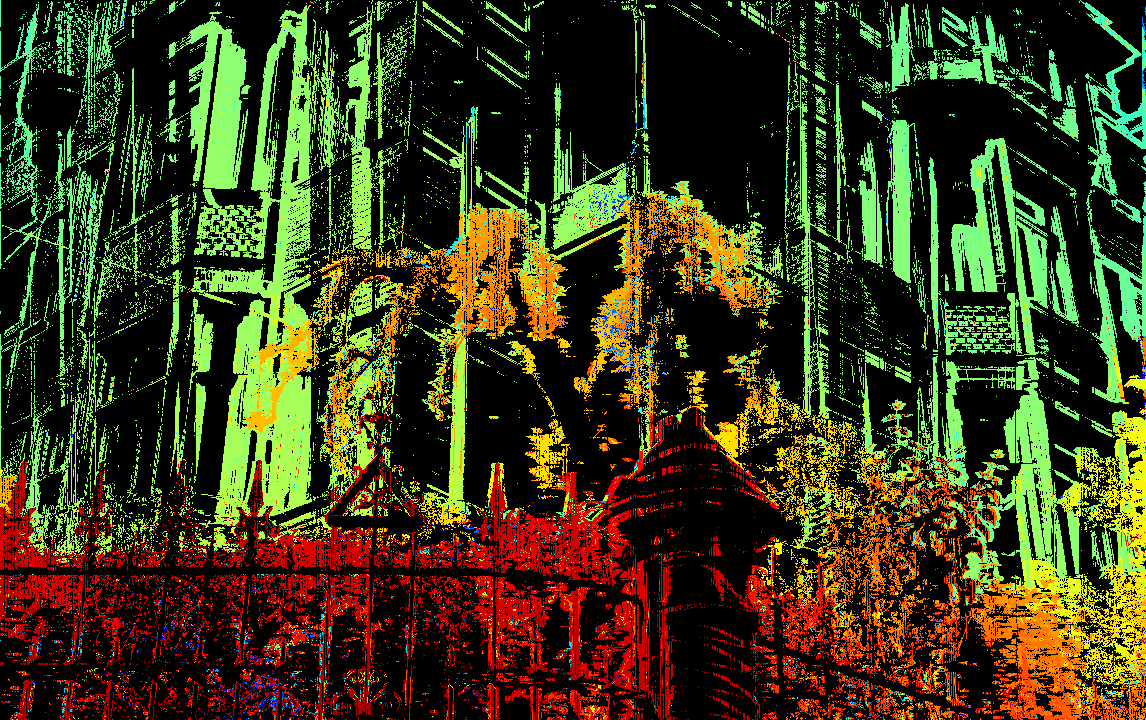
\includegraphics[width=0.6\textwidth]{images/1520973007982_dmap_025.png}
  \caption{Disparity map (frame 25), when popagating only the points with $C_d > 0.1$ and displaying only points with $C_d > 0.1$. We see that there seem to be more outliers than on the previous Figure (and less points drawn overall) ; it might be that the propagation is a way of ensuring consistency between frames, and thus reducing this effect. We can assume nonetheless than the $d$ values are more precise on the points on the wall of the mansion than on the previous Figure.}
  \label{fig:propagation:disp}
\end{figure}

%\begin{figure}[ht]
%  \centering
% \animategraphics[autoplay,loop,width=0.5\textwidth,controls]{5}{animate_skysat/1520867757275_dmap_}{000}{100}
%\end{figure}




\clearpage
\bibliographystyle{plain}
\bibliography{bibliography}


\end{document}